\documentclass[11pt]{article}
\usepackage[final]{graphicx}
\usepackage{times}

\setcounter{secnumdepth}{3}
\setcounter{tocdepth}{3}

\usepackage{url}
\usepackage[colorlinks, bookmarks=true]{hyperref}

\makeatletter
\def\url@smallurlstyle{%
  \@ifundefined{selectfont}{\def\UrlFont{\sf}}{\def\UrlFont{\small\ttfamily}}}
\makeatother
\urlstyle{smallurl}

\usepackage{xspace}
\newcommand{\COtwo}{CO\ensuremath{_2}\xspace}

\usepackage{fullpage}

\usepackage{floatflt}
\usepackage{wrapfig}

%\usepackage{breakurl}

\begin{document}
\title{OPQ Cloud: A scalable software framework for the aggregation of distributed power quality data}
\author{Anthony J. Christe \\
      Collaborative Software Development Laboratory \\
      Department of Information and Computer Sciences \\
      University of Hawai'i,  Honolulu, HI 96822 \\
      achriste@hawaii.edu}
\maketitle
%%%%%%%%%%%%%%%%%%%%%%%%%%%%%% -*- Mode: Latex -*- %%%%%%%%%%%%%%%%%%%%%%%%%%%%
%% abstract.tex -- 
%% Author          : Joseph Dane
%% Created On      : Fri Oct  8 21:04:34 1999
%% Last Modified By: Joe Dane
%% Last Modified On: Wed Oct 20 12:15:34 1999
%% RCS: $Id$
%%%%%%%%%%%%%%%%%%%%%%%%%%%%%%%%%%%%%%%%%%%%%%%%%%%%%%%%%%%%%%%%%%%%%%%%%%%%%%%
%% Copyright (c) 1999 Joseph Dane
%%%%%%%%%%%%%%%%%%%%%%%%%%%%%%%%%%%%%%%%%%%%%%%%%%%%%%%%%%%%%%%%%%%%%%%%%%%%%%%
%% 

\begin{abstract}

  Effective program size measurement is difficult to accomplish.  Factors
  such as program implementation language, programmer experience and
  application domain influence the effectiveness of particular size metrics
  to such a degree that it is unlikely that any single size metric will be
  appropriate for all applications. This thesis introduces a tool, LOCC,
  which provides a generic architecture and interface to the production and
  use of different size metrics.  Developers can use the size metrics
  distributed with LOCC or can design their own metrics, which can be
  easily incorporated into LOCC.  LOCC pays particular attention to the
  problem of supporting incremental development, where a work product is
  not created all at once but rather through a sequence of small changes
  applied to previously developed programs.  LOCC requires that developers
  of new size metrics support this approach by providing a means of
  comparing two versions of a program.  LOCC's effectiveness was evaluated
  by using it to count over 50,000 lines of Java code, by soliciting
  responses to a questionnaire sent to users, and by personal reflection on
  the process of using and extending it.  The evaluation revealed that
  users of LOCC found that it assisted them in their development process,
  although there were some improvements which could be made.


\end{abstract}

\tableofcontents
\listoftables
\listoffigures
\newpage
\section{Introduction and Motivation}
According to the Office of Electricity Delivery \& Energy Reliability, the electricity that we consume in the United States should have a frequency of 60 Hz and a voltage of 120 V \cite{OEDER}. Power quality (PQ) issues arise whenever there is a deviation from these standards or when other harmonics get introduced into the power.

Common PQ issues include voltage sag, voltage flicker, and harmonics.   \cite{atputharajah}. For our current OPQ project, we're only measuring voltage and frequency. However, we plan to study the affects of harmonics through total harmonic distortion (THD) in the future.

We're initially focusing our research efforts on the state of Hawaii. Hawaii is currently in a state of transition changing its electrical grid from its current 90\% fossil fuels / 10\% renewables to 60\% fossil fuels / 40\% renewables by 2030 \cite{hawaii-mandate}. Consumers and businesses are installing photovoltaics at increasingly high rates \cite{pv-rates}. Common issues that can occur with renewables on the grid include undervoltage, overvoltage, output power fluctuation, harmonic distortion, and frequency fluctuation \cite{Farhoodnea}. Because of this, consumers are running into roadblocks by way of the utility companies due to possible grid instabilities that can arise with renewable energy sources \cite{pv-pushback} being introduced to the power grid. 

A major problem is that there is no data that consumers can point to that says ``hey, the power quality in our neighborhood is good, so we should be able to install photovoltiacs. Instead consumers only know what they're told by the utilities. Even then, utilities are not mandated to report on PQ information.

On the flip side, distributed PQ data does not exist for the utilities either, and they have to force consumers to wait until their neighborhood can be studied by utility engineers to ensure that the addition of renewables is not going to harm the grid.

Power quality also has an effect on large industries' bottom lines. Laskar et al. found that voltage fluctuations can damage sensitive electronic equipment and can cost companies quite a lot of money. For example, a semiconductor production plant will lose over 5 million USD per power event. Financial trading companies will lose over 8 million USD an hour during power events \cite{Laskar}. It's important to note that these are just power events, not power outages. It's important for companies to understand the PQ that is coming into their plants and to also understand the PQ of the neighborhoods around them and how that PQ can affect their bottom line.

\section{A Software and Hardware Diagnostic Framework}
Our project contains a hardware devices for measuring voltage and frequency and also a software framework for aggregating distributed PQ measurements and events. The software framework is the focus of this paper.

The OPQ project provides a software solution which aggregates crowd sourced distributed PQ data. We provide real time monitoring and alerts for users when PQ events occur. We also provide a simple wizard style sign up which allows users to connect to their OPQ hardware devices with ease. Users can manage their PQ data in an intuitive and anonymous way. Users can also receive alerts via email or SMS.

Our project is built using a large selection of open source technologies. For a full list of software and libraries used in our project, see section \ref{software_used}. 

We believe that our system can provide crowd sourced distributed PQ data to consumers, businesses, and utilities alike. We hope to provide a transparent way of collecting and distributing PQ data. We want to empower consumers to understand the quality of the power feeding into their homes and to understand the PQ of the neighborhood they reside in. Businesses should be able to safeguard their electrical assets by assessing the possible threats to their company due to PQ. We want utilities to have a better understanding of PQ so that they can work with correcting PQ issues. Utilities can also use our data to stand out-of-the-way of renewables when there aren't PQ issues. We believe that the OPQ project is a step closer to realizing a smarter grid.

One of the main tenants of our project is openness. We provide openness in three ways. Our software is built on top of open source libraries. Our software is itself released under an open source license (GPL v3), and our data is open so that other researchers and the public can make informed decisions about PQ.

\section{Software Implementation}
\subsection{Obtaining the Software}
All software and related documentation for our project can be found at OPQ's github page \url{<https://github.com/openpowerquality/>}.

\subsection{Grid Map}
A useful tool when working with geographically distributed data is a dynamic map to visualize PQ events and other PQ related information. We're using the Leaftlet Javascript library to provide a mapping interface. For the actual map imagery, we're using the open licensed OpenStreetMap tiling images.

Leaflet provides utilities for placing markers and icons, and we heavily used this early on to display the location of PQ events. We realized that this approach caused several issues. First, we do not want to compromise our users' privacy by displaying the exact location of their OPQ device on a map. Second, if multiple PQ events happen near each other, the map would become cluttered with icons.

We came up with an approach that allows users to select their own level of anonymity while still providing useful and easy to parse visual information.

The Leaflet library allows the for creation of polygon layers where the points of the polygon can be encoded in JSON. We created a Javascript grid-map library which utilizes Leaflet's polygon layer and splits the map up into a series of evenly divided grid squares (similar in idea to a checker board). We wrapped this functionality up into a library using the Javascript module pattern to separate the public API from the back end code. This library allows us to use our map interface in separate locations in our cloud service.

\subsubsection{Generating the Polygon Points}
To generate an evenly spaced grid, we identified the NW and SE latitude and longitude points of the bounding box (BB) that contains the area of interest our grid should cover. The BB we chose for Hawaii is outlined in table \ref{tab:bb_hawaii}.

\begin{table}[htbp]
	\caption{Hawaii Grid Square Bounding Box}
	\label{tab:bb_hawaii}
	\begin{center}
		\begin{tabular}{|l|r|r|r|}
			\hline
			\textbf{BB Point} & \textbf{ Location} & \textbf{Latitude} & \textbf{Longitude}\\
			\hline
			North West & NW of Niihau & 22.534353 & -161.004639\\
			\hline
			South East & SE of Big Island & 16.719592 & -151.853027\\
			\hline
		\end{tabular} 
	\end{center}
\end{table}

We can calculate the latitude ($\phi$) and longitude ($\lambda$) of a point $(\phi_2, \lambda_2)$, given a starting point $(
\phi_1, \lambda_1)$, bearing ($\Theta$), distance ($d$), and angular distance ($AD=\frac{d}{radius\ of\ earth}$) with the following formula which uses the distance over a great arc circle as an approximation for the shape of the earth.

$\phi_2 = asin(sin(\phi_1 * cos(AD) + cos(\phi_1) + sin(AD) * cos(\Theta))$

$\lambda_2 = \lambda_1 + atan2(sin(\Theta) * sin(AD) * cos(\phi_1), cos(AD) - sin(\phi_1) * sin(\phi_2))$

With the above formula, we start with the NW point of the BB, and generate all points due South of the starting point within the BB with a given distance interval. This process generates the first point for each of the row in our point matrix. Then for each starting point, we generate all points due East within the BB. The result of this process is a matrix of evenly spaced points which can then be used to create polygons of evenly spaced grid squares. It should be noted that we optimize our library so that only polygons within the current browser window viewing area are generated.

\subsubsection{Dynamic Sizing of Grid}
Grid scale is defined as the length of each square polygon in the grid. That is, a grid scale of 256 kilometers contains grid squares which each are 256 kilometers by 256 kilometers. The coarsest grid scale that we support is 256 kilometers and the finest grid scale is $\frac{1}{8}$ kilometer.

We designed our grid-map library so that when the map is zoomed out, it displays the coarsest grid of 256 kilometers. As the map is zoomed in, each grid square is recursively divided into four smaller squares, each with a grid-scale that is exactly one-half of its parent's. This process continues until the map is at max zoom and each grid square represents $\frac{1}{8}$ of a kilometer.

The location of any grid is invariant to both zoom and pan as long as the NE BB starting point is not changed. This makes it easy to associate ids with individual grid squares so that devices can then be associated with individual grid squares.

\subsubsection{Grid Square Naming}
In order to associate OPQ hardware devices with locations on the grid, we developed a naming scheme that stores the parent information of each grid in the name itself. Grids at the coarsest grid scale (256 kilometers) are simply named by their row ($r$) and column ($c$) using the format $r,c:$. We show  an example of how the coarsest grid squares would be named in figure \ref{fig:coarsest_grid_ids}.

\begin{figure}[htbp]
	\centering
	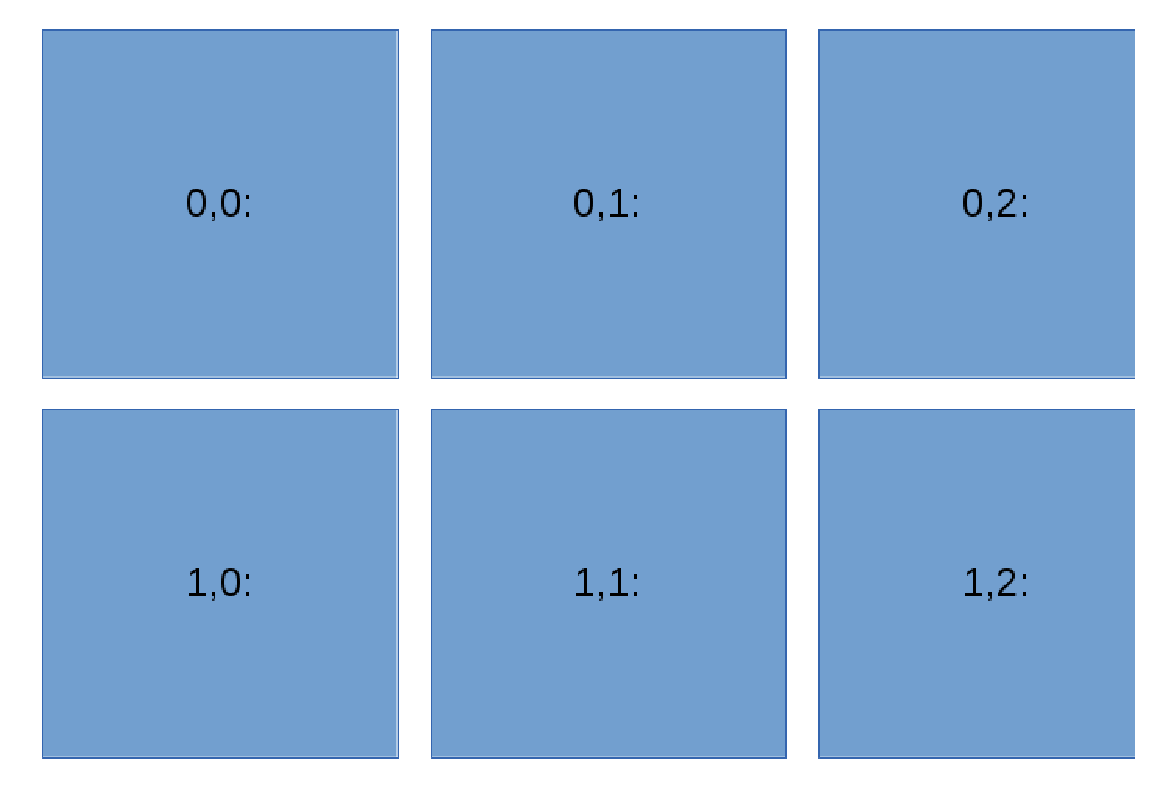
\includegraphics[width=0.8\textwidth]{figures/grid-sq.eps}
	\caption{Naming Convention for Coarsest Grid Layer.}
	\label{fig:coarsest_grid_ids}
\end{figure}

For each level that the grid becomes more fine, each square recursively divides into four squares. We can name each of these child squares by its location in the parent square. For each finer level, we simply append this location id onto its parent's id.

\begin{table}[htbp]
	\caption{Naming of Child Grid Squares}
	\label{tab:grid_first_child}
	\begin{center}
		\begin{tabular}{|l|r|}
			\hline
			\textbf{Position in Parent} & \textbf{ID}\\
			\hline
			Top Left & 0\\
			\hline
			Top Right & 1\\
			\hline
			Bottom Right & 2\\
			\hline
			Bottom Left & 3\\
			\hline
		\end{tabular} 
	\end{center}
\end{table}

Figure \ref{fig:first_children} shows the ids of the first level of children under the parent grid square.

\begin{figure}[htbp]
	\centering
	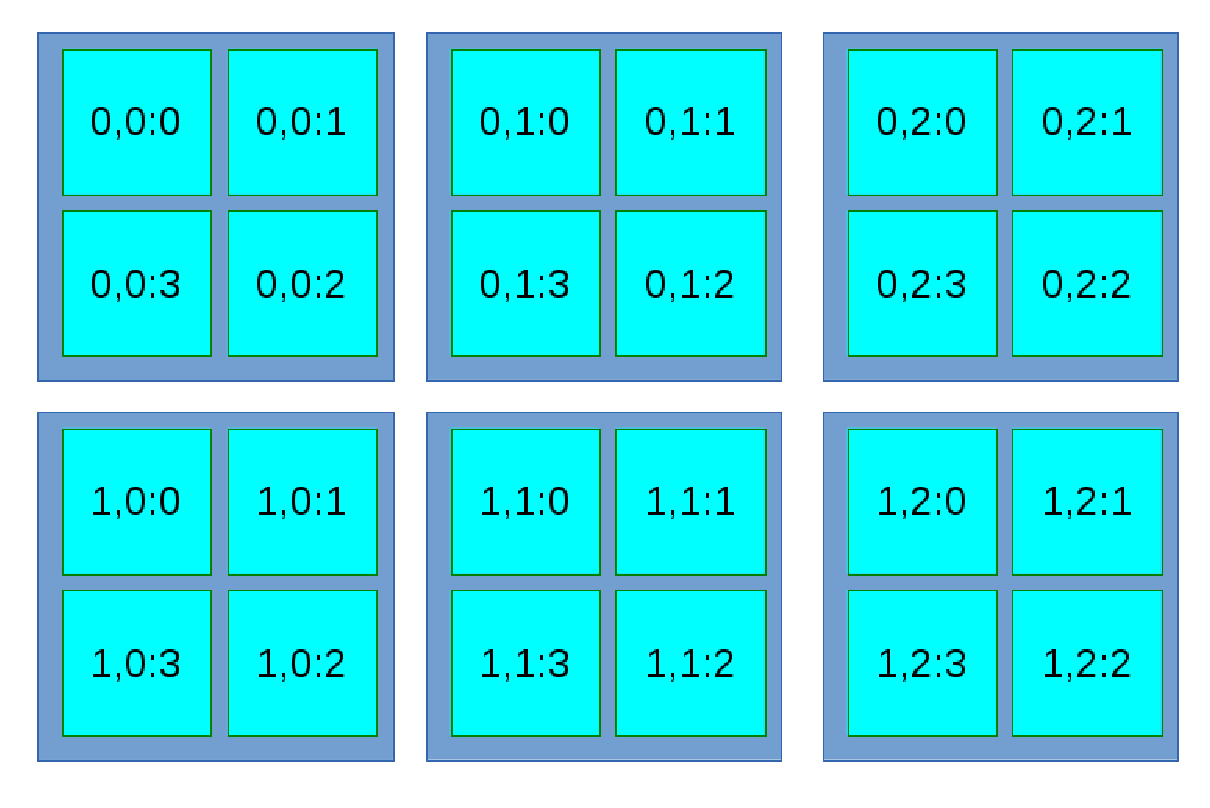
\includegraphics[width=0.8\textwidth]{figures/grid-sq-1.eps}
	\caption{Naming Convention for First Children.}
	\label{fig:first_children}
\end{figure}

We can then recursively use the same naming scheme for each level of children in the grid. For example, a grid id of ``0,0:13" represents the following information. At the coarsest level, the location ``0,0:" represents the top left 256x256 kilometer grid square. The following ``1" represents that the 128x128 kilometer child of the coarsest level is located at the top right of its parent square. The following ``3" represents that the grandchild of the coarsest square is in the bottom left of the child's square. To illustrate the concept of recursive ids, please refer to \ref{fig:second_children}.

\begin{figure}[htbp]
	\centering
	\includegraphics[width=0.8\textwidth]{figures/grid-sq-2.eps}
	\caption{Recursive Naming of Children.}
	\label{fig:second_children}
\end{figure}

\subsubsection{Importance to OPQ}
We want our users to feel comfortable sharing their PQ information. We want to empower our users to select the amount of anonymity they require when sharing the location of their OPQ hardware device. Our grid system allows users to select any grid square at any grid scale for the location of their device. This means that if a user is comfortable giving away the relative location of their home, they can select a $\frac{1}{8}$ kilometer grid square which contains their device. If they are not as comfortable with such an accurate location, they can choose a larger grid square, perhaps $\frac{1}{2}$ kilometer, 2 kilometers, 4 kilometers, etc.

We can also use the user's defined location to determine their local PQ neighborhood. A user is said to be part of a neighborhood if they've selected their location with a grid scale of less than or equal to 4 kilometers. Their neighborhood is all parent grid squares up to and including 4 kilometers.

\subsection{OPQ Cloud Features}
\subsubsection{Sign-Up}
Our sign up process collects information about the owner of an OPQ hardware device as well as information about the device itself. We use a custom wizard style dialogue provided by Fuel UX to make it easy for users to set up their device(s). 

After collecting the user's contact information, the wizard associates the user's account with their OPQ hardware device(s). To do this, we ask for the provided id number of the OPQ device(s). After the device is associated with the user's account, we allow the user to opt-in to our data sharing program by selecting their approximate location on our grid-map. This feature makes it possible to anonymously share your PQ data with the community. Finally, we collect the user's SMS and preferred contact email so that users can be alerted by email, SMS, or both when PQ events take place.

Examples of our sign up wizard can be found in the attached screenshots as figures \ref{fig:wizard_1}, \ref{fig:wizard_2}, \ref{fig:wizard_3}, \ref{fig:wizard_4}, \ref{fig:wizard_5}, and \ref{fig:wizard_6}.

\subsubsection{PQ Measurements}
Our measurements section shows 20 voltage and frequency measurements per page. The measurements are ordered by most recent. The user is able to select which of their devices they want to show PQ measurements for. Users can also filter measurements by the last minute, hour, day, week, month, year, or all. 

An example of our measurements page can be found in the attached screenshots as figure \ref{fig:private_measurements}.

\subsubsection{PQ Events}
The PQ events page is the first page a user is redirected to after logging in. This page shows  20 PQ events per page from all the user's devices. The events are ordered by most recent first. This page shows the type of PQ event (frequency, voltage, or device), the value of the event (i.e. 65 Hz), the timestamp of the event, and the duration of the event (i.e. 2000 milliseconds). Users can also filter events by the last minute, hour, day, week, month, year, or all.

This page also allows users to tag PQ events with an external cause. For instance, possible tags might include ``downed power line", ``tropical storm Flossie", or ``refrigerator condenser". 

An example of the PQ Events page can be found in the attached screenshots as figure \ref{fig:private_events}.

\subsubsection{Data Sharing}
OPQ users are able to share their PQ information by opting in to our community data sharing program. In order for a user to share their data, they simply select the finest grid scale their comfortable with that their OPQ device resides in. When users share their data, they also get access to nearby PQ events from other users sharing their data within the same neighborhood. Users may complete this process during sign up, or opt-in (or out) at any later time.

\subsubsection{Nearby PQ Events}
OPQ users in the same neighborhood can receive alerts about PQ events within their neighborhood. A neighborhood is chosen by the user when they select to share their data and select the appropriate grid square for their device. A neighborhood is defined as the user's selected grid square and all parent squares up to 4 kilometers. 

An example of our device administration page can be found under the attached screenshots as figure \ref{fig:nearby_events}.

\subsubsection{Device Administration}
With our device administration page, users can easily add more OPQ devices to their profile or update details about existing devices that they own. Users can give nicknames to devices such as ``lab", ``garage", or ``warehouse \#3" so that they don't have to memorize the id number of each device. Users can also customize the types of PQ alerts they receive during PQ events for each device. They can define the e-mail and SMS number for alerts per device.

An example of our device administration page can be found under the attached screenshots as figure \ref{fig:device_admin}.

\subsection{OPQ Cloud Infrastructure}
\subsubsection{Database Design}
We're using the Ebean ORM for persistence throughout our cloud service. Ebean is backed using a MySQL database. The persisted entities in our software are described in table \ref{tab:persisted_entities}.

\begin{table}[htbp]
	\caption{Persisted Entities}
	\label{tab:persisted_entities}
	\begin{center}
		\begin{tabular}{|l|r|}
			\hline 
			\textbf{Entity} & \textbf{Description} \\ 
			\hline 
			Alert & User defined e-mail or SMS alert. \\ 
			\hline 
			Event & A PQ event. \\ 
			\hline 
			ExternalCause & A user tagged external cause (i.e. tropical storm). \\ 
			\hline 
			Measurement & A single frequency and voltage measurement. \\ 
			\hline 
			OpqDevice & A single OPQ hardware unit's information. \\ 
			\hline 
			Person & A single owner of an OPQ hardware device. \\
		\hline
		\end{tabular} 
	\end{center}
\end{table}

The table structure is described as a Crow's Foot ER diagram in figure \ref{fig:db_er_diagram}.

\begin{figure}[htbp]
	\centering
	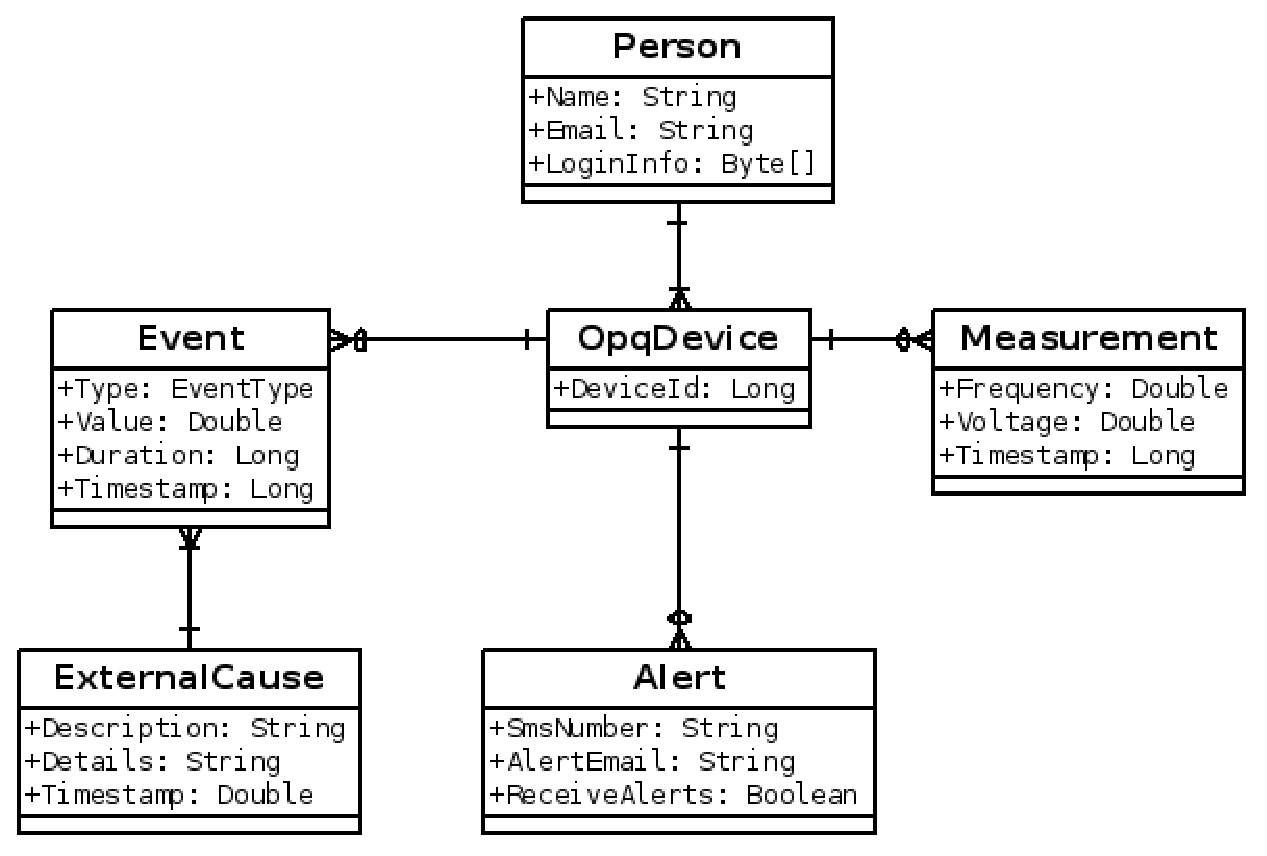
\includegraphics[width=0.8\textwidth]{figures/db.eps}
	\caption{Crow's Foot DB ER diagram.}
	\label{fig:db_er_diagram}
\end{figure}

\subsubsection{Asynchronous 2-Way Communication}
Not only can OPQ hardware devices send information to the OPQ cloud service, but the OPQ cloud service also has the infrastructure to send or request information from OPQ devices. In order for the cloud service to send or request information from OPQ devices, the OPQ devices first have to ping the cloud service to tell the cloud service that that device exists and is online. 

This is achieved when the cloud service receives a ping packet from an OPQ device, and then creates a mapping from that device's ID to the WebSocket handler associated with that device. 

When the cloud service needs to contact the device, it looks up the appropriate WebSocket handler from the map, and then uses that WebSocket handler to communicate with the device.

Devices are pruned from the mapping if they have not sent any data for over an hour. 

\subsection{OPQ Protocol}
We've created a custom communication protocol between OPQ devices and our OPQ cloud service. Our OPQ simulator also makes use of our OPQ communication protocol. Our protocol utilizes a fixed length header with a variable sized payload. The layout of the protocol is described below.

\begin{table}[htbp]
	\caption{Protocol Layout}
	\label{tab:protocol_layout}
	\begin{center}
		\begin{tabular}{|l|r|r|r|r|}
			\hline 
			\textbf{Description} & \textbf{Size (bytes)} & \textbf{Start Byte} & \textbf{End Byte}\\ 
			\hline 
			Magic Word Header & 4 & 0 & 3\\ 
			\hline 
			Type & 4 & 4 & 7\\ 
			\hline 
			Sequence Number & 4 & 8 & 11\\ 
			\hline 
			Device Id & 8 & 12 & 19\\ 
			\hline 
			Timestamp & 8 & 20 & 27\\ 
			\hline 
			Bitfield & 4 & 28 & 31\\ 
			\hline 
			Payload Size & 4 & 32 & 35\\ 
			\hline 
			Reserved & 16 & 36 & 51\\ 
			\hline 
			Checksum & 4 & 52 & 55\\ 
			\hline 
			Payload & Variable & 56 & 56 + P\\ 
			\hline 
		\end{tabular}
	\end{center}
\end{table} 

\subsubsection{Magic Word Header}
The magic word header is simply 4 bytes which signify the start of an OPQ data packet. The four bytes will always be 0x00C0FFEE.

\subsubsection{Type}
The type field specifies the type of OPQ packet being sent. The types and their values are specified below. 

\begin{table}[htbp]
	\caption{Packet Types}
	\label{tab:packet_types}
	\begin{center}
		\begin{tabular}{|l|r|r|}
			\hline
			\textbf{Type} & \textbf{Value} & \textbf{Description}\\
			\hline
			Measurement & 0 & Frequency and voltage measurement.\\
			\hline
			Frequency Event & 1 & This packet contains frequency PE data.\\
			\hline
			Voltage Event & 2 & This packet contains voltage PE data.\\
			\hline
			Device Event & 3 & This packet contains device event data.\\
			\hline
			Ping & 4 & Establishes connection with OPQ cloud (no payload).\\
			\hline
		\end{tabular}
	\end{center}
\end{table} 

\subsubsection{Sequence Number}
The sequence number is a 4 byte field which maintains the ordering of packets in multi-packet transmissions. This way, if packets are received out-of-order, they can be reassembled in the correct order.

\subsubsection{Devive Id}
This field represents a positive 64-bit integer which uniquely identifies each OPQ hardware device. 

\subsubsection{Timestamp}
This field is a 64-bit integer which represents the number of milliseconds since the epoch of when this packet was sent.

\subsubsection{Bitfield}
This is a 4-byte bitmask where each bit represents one of 32 options depending on the type of packet. This is currently not being used, but it's use is planned for future expansion.

\subsubsection{Payload Size}
A 32-bit integer which stores the size of the payload for each packet.

\subsubsection{Reserved}
These 16-bytes are reserved for later use.

\subsubsection{Checksum}
The checksum of each packet is a 4-byte field that is computed by summing every field in the packet except for the checksum field itself. In other words, the checksum $C$ is computed as $C=sum(all\ bytes) - sum(bytes[52-55])$. 

\subsubsection{Payload}
The payload is a variable length field which contains different data depending on the type of packet being sent. The three types of payloads are described below.

If the packet is a measurement type, the payload is 16 bytes where the first 8 bytes represent an IEEE 754 floating point number of the frequency and the last 8 bytes represent an IEEE 754 floating point number of the voltage.

If the packet is a frequency event type, the payload is 16 bytes where the first 8 bytes represent an IEEE 754 floating point number of the frequency and the last 8 bytes represent the duration of the event as a 64-bit long integer. The duration represents the number of milliseconds since the epoch.

If the packet is a voltage event type, the payload is 16 bytes where the first 8 bytes represent an IEEE 754 floating point number of the voltage and the last 8 bytes represent the duration of the event as a 64-bit long integer. The duration represents the number of milliseconds since the epoch.

If the packet type is a ping packet, the payload remains empty.

\subsection{Reference Implementation of Protocol}
A fully tested reference implementation of our protocol has been written as a standard Java library. We're currently using this implementation of the protocol is both our OPQ simulator and our OPQ cloud service.

The reference implementation provides many utilities which aid in the construction of OPQ packets. For example we provide convenient getters and setters that accept decimal inputs for frequency, voltage, device id, event duration, timestamp, etc.

The setters convert the decimal values into the appropriate array of bytes and stores them at the correct location in the protocol. The setters also make sure that the payload section of the protocol is structured correctly. 

The getters select the correct subarray of bytes from the protocol and converts them into a readable decimal value.

The library itself is resilient against inadvertently creating invalid packets. The library contains a wide range of custom exceptions which are thrown when an OPQ packet is put into an invalid state.

\subsection{OPQ Simulator}
We designed an OPQ hardware simulator so that we could try out new ideas without needing to deploy actual hardware right away. Our OPQ simulator can act as a proxy for a real OPQ hardware device or as a proxy for many OPQ devices. Utilizing our reference implementation of the OPQ protocol, the OPQ simulator simulates actual OPQ data packets.

We provide a GUI designed using the JavaFX framework which allows for fined grained control over sending a single OPQ packet, or for the implementation of various distributed simulations.

\subsubsection{Single Packet Simulation}
When testing our OPQ Cloud service, we found that we needed the ability to send single OPQ packets to the cloud service where we could control all details of the packet being sent. We provide an interface that makes it easy to construct a single OPQ packet and then send it to cloud service for evaluation. We also provide the functionality to alter your values in both decimal and hexadecimal notations at the same time.

Users of the simulator can alter the fields described in table \ref{tab:single_packet_sim}.

\begin{table}[htbp]
	\caption{Single Packet Simulation Fields}
	\label{tab:single_packet_sim}
	\begin{center}
		\begin{tabular}{|l|r|}
			\hline
			\textbf{Field} & \textbf{Details}\\
			\hline
			Websocket URL & URL of cloud service.\\
			\hline
			Device Id & The simulated OPQ hardware device id.\\
			\hline
			Type & One of the available OPQ packet types.\\
			\hline
			Sequence Number & Sequence number for simulated multi-packet data.\\
			\hline
			Timestamp & The number of milliseconds since the epoch.\\
			\hline
			Bitfield & Bitfield options for the simulated packet.\\
			\hline
			Frequency & The frequency of the simulated packet.\\
			\hline
			Voltage & The voltage of the simulated packet.\\
			\hline
			Alert Duration & The duration of the simulated event.\\
			\hline
		\end{tabular}
	\end{center}
\end{table} 

The GUI makes it difficult to create invalid OPQ packets. For example, when the type of packet is ``Event Frequency", the fields for modifying the voltage become uneditable and set to 0. If the type of packet is ``Event Voltage", the frequency fields become uneditable. When the type of packet is ``Measurement", then the duration field is made uneditable. If the type of packet is ``Ping", then only the device id and timestamp fields remain editable. An example of the single packet simulation can be seen in figure \ref{fig:sim_single}.

\subsubsection{Distributed Simulations}
Our OPQ simulator also provides a simulation for performing single-source, large-data testing on our OPQ cloud service. The simulation allows for a variable number of devices which continually send measurements and generate PQ events a definable percentage of the time. For a more accurate simulation, a thread is generated for each device, so that their packet timing is independent of other devices.

A description of the editable fields are provided in table \ref{tab:dist_sim}.

\begin{table}[htbp]
	\caption{Distributed Simulation Fields}
	\label{tab:dist_sim}
	\begin{center}
		\begin{tabular}{|l|r|}
			\hline
			\textbf{Field} & \textbf{Details}\\
			\hline
			Websocket URL & URL of cloud service.\\
			\hline
			Device Ids & List of OPQ device ids to send packets from.\\
			\hline
			Packet Types & Any available OPQ packet types (except ping).\\
			\hline
			Packets/second & The number of packets each device sends per second.\\
			\hline
			Event Frequency & Percentage between [0.0 - 1.0].\\
			\hline
		\end{tabular}
	\end{center}
\end{table} 

Note that the ``Event Frequency" field determines how frequency a PQ event should be generated by each device. A value of .5 would say that each device should generate a PQ event 50\% of the time, whereas a value of .1 says that each device should only generate PQ events 10\% of the time. An example of this simulation can be seen in figure \ref{fig:sim_multi}.

\section{Evaluation and Results}
\subsection{Using the OPQ Simulator}
We used the OPQ simulator to send simulated measurements and PQ events to the OPQ cloud service. We tested that the measurements and events received by the cloud service were the same ones sent by the simulator. We did this for multiple users and multiple simulated devices.

Users that were set up to receive SMS and/or email alerts received those alerts when PQ events were generated by the simulator. Users who opted to share their PQ data also received alerts that were generated within their neighborhood. 

\subsection{Performance and Scalability}
Our hosting provider Cloudbees provides a service called New Relic which provides application performance management. In other words, New Relic is an online service attached to Cloudbees which can perform profiling on our OPQ cloud service. We found the following metrics for our cloud based service to be the most telling at our current stage of the project.

\subsubsection{Response Time}
There are three categories for response times that developers need to concern themselves with. Less than 0.1 seconds feels instantaneous to users. Less than 1.0 second is the limit for a user's flow of thought to go uninterrupted, and less than 10 seconds keeps the user's attention \cite{response-time}. 

In order to calculate response time, we navigated all sections of our cloud service under normal simulated load from OPQ devices.

Our software when selecting a link and seeing an updated page has an average response time of 289 milliseconds with the largest response time being just under 750 milliseconds. Our response time falls just between the two categories of instantaneous and keeping the user's train of thought. As long as our response times remain less than a second, then no large architectural changes need to made to accommodate faster response times.

The 750 millisecond response time is generated when loading the page that describes PQ events. The reason for the high response time is due to database calls which access all power events associated with all devices for the particular user. Even though the events page causes the highest response time, since the response time is less than a second, we're currently not concerned with it. Further analysis on the database response time is discussed in the next section, database profiling.

The response time for both our web service and for our database are described in figure \ref{fig:response_time}.

\begin{figure}[htbp]
	\centering
	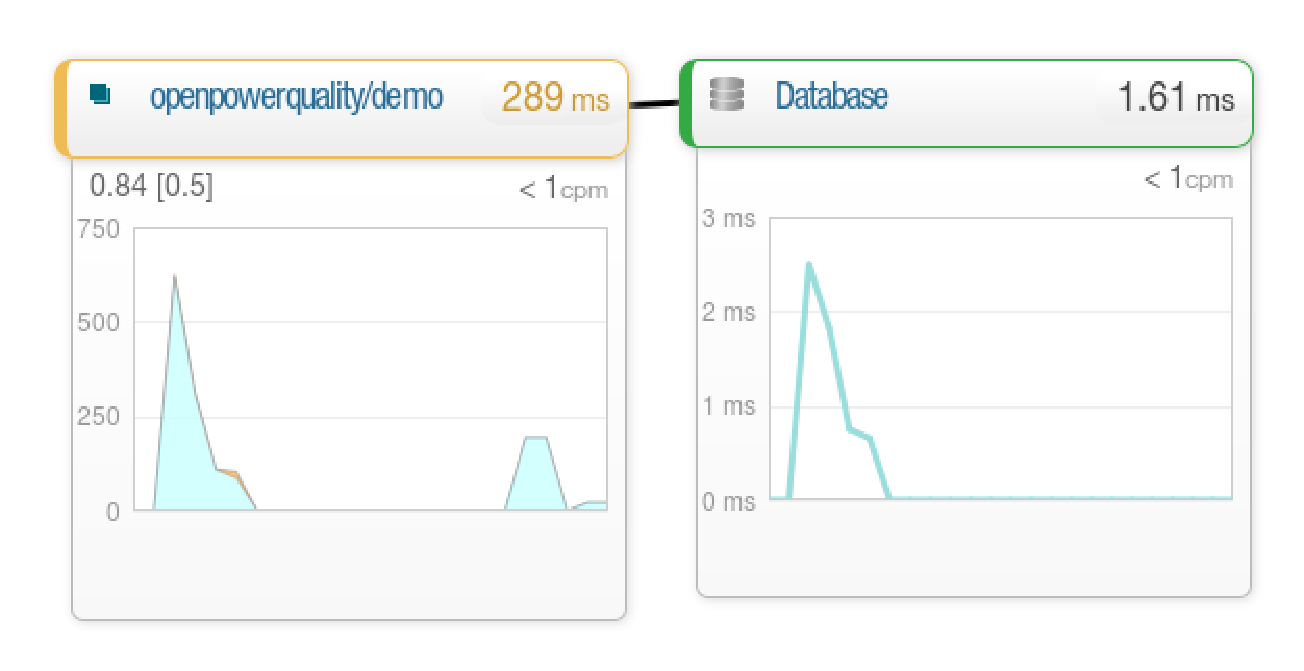
\includegraphics[width=0.8\textwidth]{figures/response_time.eps}
	\caption{Web Service and DB Response Times.}
	\label{fig:response_time}
\end{figure}

\subsubsection{Database Profiling}
We stress tested our Cloudbees database using our OPQ simulator with a simulation of 20 OPQ devices each sending either measurements or PQ events five times a second. In other words, our webservice and database was responding to and storing 100 OPQ packets per second. We chose this for our initial stress testing as it's our aim for our initial pilot deployment of devices.

We found that stress testing the database with the above parameters would use about 5 megabytes of data in half an hour. Extrapolating this data, our service will consume about 240 megabytes a day, 1.7 gigabytes a week, and 6.7 gigabytes per month. This number can be greatly reduced if we only send occasional measurements and PQ events when they occur instead of multiple measurements per device per second.

When profiling the database we can provide several metrics. 

The top five most time consuming database operations are outlined in table \ref{tab:db_response}.

\begin{table}[htbp]
	\caption{Database Profiling}
	\label{tab:db_response}
	\begin{center}
		\begin{tabular}{|l|r|r|r|}
			\hline
			\textbf{DB Field} & \textbf{Operation} & \textbf{Total \% of Time} & \textbf{Avg. Response Time (ms)}\\
			\hline
			OPQ Device & Select & 52.4 & 2.41\\
			\hline
			Person & Select & 19.9 & 3.82\\
			\hline
			Event & Select & 19.4 & 8.18\\
			\hline
		    Measurement & Select & 7.16 & 3.78\\
			\hline
			OPQ Device & Insert & 0.66 & 1.4\\
			\hline
		\end{tabular}
	\end{center}
\end{table} 

Even though querying OPQ devices takes up the largest amount of time in the database, the average response time is still less than 0.1 seconds which is well within the responsive zone that we're aiming for.

\section{Future Work}
\subsection{External Causes}
Users have the ability to tag PQ events with external causes if the user knows what caused the PQ event. Currently, users can tag events for their own records, but this feature could lead us to some interesting analytics.

We hope utilize this feature with possibilities of crowdsourcing common tags to diagnose an entire neighborhood containing PQ events. One example would be if there is a bad storm and the PQ fluctuates in the area under that storm. Users could tag their PQ events as related to the storm, and we could basically track the path of the storm by following the tags. 

Eventually, we would like to employ machine learning to infer information from user defined tags. If a user sees that they have a power event every time their refrigerator turns on, they can tag the event with their refrigerator model and machine learning can learn to associate that PQ signature with the turning on of that particular compressor. With that learned fact, we can filter and identify these signatures in all homes. In this way, we could classify PQ event signatures with the help of crowdsourcing.

Once we're able to classify power events through machine learning, we can provide recommendations to users on how they can mitigate their PQ issues that we diagnosed. If we can determine what constitutes as sustained PQ issues, we might be able to recommend when to call the utilities, or when they might benefit from installing power conditioning equipment, or perhaps we can alert users to unplug their electronics if we can forecast poor PQ.

\subsection{Public PQ Monitoring}
We currently only support a rudimentary map interface for displaying public PQ events. If a PQ event occurs, the grid square that it's located in and all parent grid squares will change to a red coloring. 

We would like to add the ability to reflect how many power events have happened within in area but using multiple colors indicating the density of PQ events in a particular area. 

We would also like to perform aging on PQ events so that only the most recent (being user defined) events would show up on the public map. 

Finally, we would like to provide an animated map interface that would should cascading PQ events. The inspiration behind this is similar to weather maps which can show the animated path of a storm, we would like to show an animated path of PQ events. 

\subsection{Security and Privacy}
The Play framework provides built-in support for SSL encryption. We are currently not encrypting our traffic, but as soon as it can be implemented in hardware and implemented in the OPQ simulator, we can enable SSL on the cloud service as well.

We believe that our grid-map approach is a step in the right direction to protecting user privacy, but we also see the need for a privacy study which will determine the amount of information that can be obtained from our OPQ project and our OPQ data. We need to determine if there are problems with our approach in terms of privacy, and if so, how can we address them?

\subsection{Usability Testing}
Our software has not undergone any usability testing. We need to perform usability testing and make changes based on those tests. We hope to begin basic usability testing as soon as we start our pilot program once we're ready to deploy our OPQ hardware devices.

\subsection{Other Event Types}
We are currently only monitoring voltage and frequency. We believe that our hardware is capable of monitoring other useful PQ metrics as well. One area that we plan on focusing on in the near future is the measuring of harmonics through total harmonic distortion (THD). We would like to study the affects of renewable power sources on the grid and how they contribute to adding harmonics on top of the power on the grid.

\subsection{Integration with Other Sources}
We would like to integrate our PQ data with power generation and consumption data by gaining access to the users utility account information.

We would also be interested in partnering with utilities and solar distribution companies to gain access to the PQ data.

\subsection{Data Analytics}
Finally, we believe that there is a myriad of data analytics that can be performed using the crowdsourced PQ data. We need to investigate the types of analytics that are possible, and then implement them. Examples of analytics that we are interested in include average neighborhood PQ, correlation of PQ with weather systems, and PQ prediction and forecasting.

\section{Conclusion}
We designed a framework of software technologies that allow for the aggregation of crowd sourced distributed PQ data. We created a cloud based service for aggregating and displaying PQ information. We created a communications protocol that we hope can become an open standard for smart meter devices. We created a grid interface that allows users to share PQ data while still remaining anonymous. We created a hardware device simulator which can be used as an analogue to a real OPQ hardware device for testing purposes. Most importantly, we laid out a solid foundation for further research.

\appendix

\chapter{Appendix}

\section{Appendix A: Game Mechanics}

The gamification wiki [ref] compiles a comprehensive list of gamification mechanics and categories them into three types (Behavioral, Feedback, Progression) and their benefits in measurable metrics (Engagement, Influence, Loyalty, User Generated Content (UGC), Time Spent, Virality) and other non-metrics ( Fun, Revenue, SEO).

\begin{table}[htbp]
  \centering
    \caption{Mega List of Game Mechanics and Benefits, part 1}
    \begin{tabular}{ | l | p {6cm} | p {4cm} | p {2cm} |}
    \hline
    Types & Mechanics / Examples & Benefits & Personality Types \\ \hline
	Progression & Achievements: normally represents as badge, completed something & Engagement, Loyalty, Time Spent, Influence, Fun, SEO, UGC & Achievers, Explorers, Killers \\ \hline
	Progression & Levels: a system of reward for a cumulation of points, Often are unlocked as players progress to higher levels. & 	Engagement, Loyalty, Influence, Time Spent, Virality, Fun & Achievers, Explorers, Killers \\ \hline
	Progression & Points: a running numerical value given for any single action or combination of actions. & Engagement, Loyalty, Influence, Time Spent, Virality, Fun, UGC & Achievers, Explorers, Killers \\ \hline
	Progression & Progression: success is granularly displayed and measured through the process of completing itemized tasks, such as a progress bar. & Engagement, Loyalty, Influence, Time Spent, Fun, UGC & Achievers, Killers \\ \hline
	Feedback & Appointment Dynamics: at a predetermined times/places a user must return for a positive effect & Engagement, Influence, Time Spent & Archivers, Explorers, Socializers \\ \hline
	Feedback & Bonuse: a reward after having completed a series of challenges or a specific task & Engagement, Influence, Time Spent, Virality, Fun, UGC & Archivers, Explorers, Socializers, Killers \\ \hline
    \end{tabular}
\end{table}

\begin{table}[htbp]
  \centering
    \caption{Mega List of Game Mechanics and Benefits, part 2}
    \begin{tabular}{ | l | p {6cm} | p {4cm} | p {2cm} |}
    \hline
    Types & Mechanics / Examples & Benefits & Personality Types \\ \hline	
	Feedback & Cascading Information Theory: information should be released in the minimum possible snippets to gain the appropriate level of understanding & Engagement, Loyalty, Influence, Time Spent & Archivers, Explorers, Socializers, Killers \\ \hline
	Feedback & Combos: reward skill through doing a combination of things, usally comes with the reward of a bonus & Engagement, Influence, Time Spent, Virality & Archivers, Explorers, Socializers, Killers \\ \hline
	Feedback & Countdown: players are only given a certain amount of time to do something. This will create an activity graph that causes increased initial activity increasing frenetically until time runs out, which is a forced extinction. & Engagement, Fun, Influence & Achievers, Explorers, Killers \\ \hline	
	Feedback & Quests/Challenges: Challenges usually implies a time limit or competition whereas Quests are meant to be a journey of obstacles a player must overcome. a way to organize player effort. & Engagement, Loyalty, Revenue, Influence, Time Spent, Virality, SEO, Fun, UGC & Achievers, Explorers, Killers \\ \hline
	Feedback & Reward Schedules: The fixed or variable timeframe and delivery of the rewards, contingency, response, reinforcer. & Engagement, Loyalty, Revenue, Influence, Time Spent, Virality, SEO, Fun, UGC & Achievers, Explorers, Killers \\ \hline
	Behavioral & Discovery/Exploration: players love to discover and to be surprised. & Engagement, Loyalty, Influence, Time Spent, Fun & Explorers, Achievers \\ \hline
	Behavioral & Epic Meaning: Players will be highly motivated if they believe they are working to achieve something great, something awe-inspiring, something bigger than themselves. & 	Engagement, Loyalty, Influence, Time Spent, Fun & Achievers, Explorers, Socializers, Killers \\ \hline
    \end{tabular}
\end{table}

\begin{table}[htbp]
  \centering
    \caption{Mega List of Game Mechanics and Benefits, part 3}
    \begin{tabular}{ | l | p {6cm} | p {4cm} | p {2cm} |}
    \hline
    Types & Mechanics / Examples & Benefits & Personality Types \\ \hline	
	Behavioral & Free Lunch: getting something for free due to someone else having done work. Groupon & Engagement, Loyalty, Revenue, Influence, Virality, Fun & Achievers, Explorers,  Socializers, Killers \\ \hline
	Behavioral & Infinite Gameplay: do not have an explicit end, static state is its own victory. & 	Engagement, Loyalty, Revenue, Influence, Time Spent, Fun & Achievers, Killers \\ \hline
	Behavioral & Loss Aversion: influences user behavior not by reward, but by not instituting punishment. the player having to perform an action to avoid losing something they currently have. & Engagement, Loyalty, Influence, Time Spent, Virality, Fun & Achievers, Explorers \\ \hline
	Behavioral & Lottery:  the winner is determined solely by chance. winners will generally continue to play indefinitely while losers will quickly abandon & Engagement, Loyalty, Revenue, Influence, Time Spent, Virality, Fun & Achievers, Explorers, Socializers, Killers \\ \hline
	Behavioral & Ownership: creates Loyalty by owning things. & Engagement, Loyalty, Revenue, Influence, Time Spent, Virality, SEO, Fun, UGC & Achievers, Explorers, Socializers, Killers \\ \hline
	Behavioral & Community Collaboration: an entire community is rallied to work together to solve a riddle, a problem or a challenge. Immensely viral and very fun. & 	Engagement, Influence, Time Spent, Virality & Archivers, Explorers, Socializers \\ \hline
    \end{tabular}
\end{table}

\begin{table}[htbp]
  \centering
    \caption{Mega List of Game Mechanics and Benefits, part 4}
    \begin{tabular}{ | l | p {6cm} | p {4cm} | p {2cm} |}
    \hline
    Types & Mechanics / Examples & Benefits & Personality Types \\ \hline	
	Behavioral & Behavioral Momentum: a tendency of players to keep doing what they have been doing & Engagement,  Loyalty, Revenue, Influence, Time Spent & Archivers, Explorers, Socializers, Killers \\ \hline
	Behavioral & Blissful Productivity: playing hard rather than relaxing makes you happier  & Engagement & Archivers, Explorers, Socializers, Killers \\ \hline
	Behavioral & Status: The rank or level of a player. Players are often motivated by trying to reach a higher level or status. Also relates to envy. & Engagement, Loyalty, Revenue, Influence, Time Spent, Virality, SEO, Fun, UGC & Achievers, Socializers,Killers \\ \hline
	Behavioral & Urgent Optimism: The desire to act immediately to tackle an obstacle combined with the belief that we have a reasonable hope of success. & Engagement, Fun & Explorers, Killers \\ \hline
	Behavioral & Virality: more successful in the game if you invite your friends, the social check-in. & Engagement, Loyalty, Revenue, Virality, SEO, UGC & Socializers, Achievers,Killers \\ \hline
    \end{tabular}
\end{table}

\section {Appendix B:  Game Elements}
Game Elements are different than mechanics, as illustrated in the examples below, they manifest the game information to the player, usually as a UI components.

\begin{table}[htbp]
  \centering
    \caption{List of Game Elements}
    \begin{tabular}{ | l | p {12cm} |}
    \hline
    Elements & Description and Examples \\ \hline
	Activity Feed & shows players what has been taking place in the system overall and motivate the player to obtain the same achievement as others. \\ \hline
	Avatars & unique representations for a player. shows a high emotional attachment between the player and the game. often customization and decoration are enhancement for higer engagement. \\ \hline
	Easter Eggs & an intentional hidden message, in-joke. \\ \hline
	Instances & are created for players to have a unique experience that is outside the normal experience. When a player creates a special unique page experience that allows to log into and view their unique content an instance has been created. \\ \hline
	Leaderboards & are a means by which users can track their performance, subjective to others. Leaderboards visually display where a user stands in regards to other users. Leaderboards can be broken down into several subcategories such as: Global, Friends, Relative, Isolated etc. \\ \hline
	The Notifier & is a direct way to give the user direct feedback about their progress, change of status in the gameplay experience etc. \\ \hline
	User Profile & displays a User's data about their activity on a website and can be used to tell the world and a community on the internet who they are. \\ \hline
    \end{tabular}
\end{table}


\bibliography{biblio}
\bibliographystyle{plain}
\end{document}
